\documentclass[12pt]{article}

% --- Packages ---
\usepackage[utf8]{inputenc}
\usepackage[T1]{fontenc}
\usepackage[french]{babel}
\usepackage{amsmath, amssymb}
\usepackage{geometry}
% \usepackage[draft]{graphicx}
\usepackage{tikz}
\usepackage[most]{tcolorbox}
\usepackage{multicol}
\usepackage{lmodern}
\usepackage{pgfplots}
\pgfplotsset{compat=1.18}
\usepackage{mdframed}
\usepackage{array}
\usepackage[thinlines]{easytable}
\usepackage{tkz-tab}
\usepackage{bm}
\usepackage{xcolor}
\usepackage{sectsty}
\usepackage[utf8]{inputenc}
\usepackage[T1]{fontenc}
\usepackage[inline]{enumitem}
\usepackage[dvipsnames]{xcolor}
\usepackage{multido}
% --- Page ---
\geometry{margin=2cm}

% Footer
\usepackage{fancyhdr}
\pagestyle{fancy}
\cfoot{\thepage}
\rfoot{\textit{G.M.}}
\renewcommand{\headrulewidth}{0pt}
\renewcommand{\footrulewidth}{0pt}

% Pour les normes : 
\newcommand*{\norme}[1]{\left\lVert\overrightarrow{#1}\right\rVert}

\usetikzlibrary{shapes.misc}

\tikzset{cross/.style={cross out, draw=black, minimum size=2*(#1-\pgflinewidth), inner sep=0pt, outer sep=0pt},
%default radius will be 1pt. 
cross/.default={4pt}}

% mettre dans le préambule, après \usepackage{xcolor}
\usepackage{sectsty} % gère facilement la couleur des titres
\setlength{\parindent}{0pt}

\sectionfont{\color{red}\Large\bfseries}     % pour \section*
\subsectionfont{\color{red}\large\bfseries\hspace{1cm}}

\begin{document}

% ============================
%   Probabilités
% ============================

\newpage

\begin{center}
    {\LARGE \textbf{Statistiques}}\\[4mm]
    {\large - 2\up{nde} -}
\end{center}

\vspace{10pt}
\hrule
\vspace{0pt}

% ============================
%   Partie 1 : Rappels sur les probabilités
% ============================

\section*{\textcolor{red}{I/ Médiane et écart interquartile}}

\subsection*{\hspace{1cm} 1) La médiane}

\vspace{5pt}

\begin{mdframed}[
    linewidth=1pt,
    roundcorner=5pt,
    linecolor=ForestGreen,
    innertopmargin=10pt,
    innerbottommargin=10pt
]
{\color{ForestGreen}
\textbf{\underline{Définition :}}}

Soit une série de $N$ valeurs rangées par ordre croissant. La \textbf{méfiane} $\bm{M}$ est le nombre défini 
par : 

\begin{itemize}
    \item si $N$ est impair, $M$ est la valeur centrale
    \item si $N$ est pair, $M$ est la moyenne des deux valeurs centrales
\end{itemize}

\end{mdframed}

\begin{mdframed}[
    linewidth=1pt,
    roundcorner=5pt,
    linecolor=Red,
    innertopmargin=10pt,
    innerbottommargin=10pt
]
{\color{red}
\textbf{\underline{Propriété :}}

\vspace{5pt}
On a ainsi moins de 50\% des valeurs de la série qui sont inférieures ou égales à la médiane.
}
\end{mdframed}

\begin{mdframed}[
    linewidth=1pt,
    roundcorner=5pt,
    linecolor=RoyalBlue,
    innertopmargin=10pt,
    innerbottommargin=10pt
]
{\color{RoyalBlue}
\textbf{\underline{Exercice d'application n°1:} Calculer une médiane}}

\vspace{5pt}
On considère la série suivante : -2 ; -1 ; 0 ; 0 ; 3 ; 4 ; 4 ; 5 ; 15 ; 25.

\vspace{5pt}
\hspace{1cm}1) Calculer l'étendue de cette série

\vspace{5pt}
\hspace{1cm}2) Calculer la médiane de la série.

\vspace{0.5cm}
{\color{black!45}\dotfill}

\vspace{0.5cm}
{\color{black!45}\dotfill}

\vspace{0.5cm}
{\color{black!45}\dotfill}

\vspace{0.5cm}
{\color{black!45}\dotfill}

\vspace{20pt}

\end{mdframed}

\vspace{10pt}
\subsection*{\hspace{1cm} 2) Les quartiles }

\begin{mdframed}[
    linewidth=1pt,
    roundcorner=5pt,
    linecolor=ForestGreen,
    innertopmargin=10pt,
    innerbottommargin=10pt
]
{\color{ForestGreen}
\textbf{\underline{Définition :}}}

\begin{itemize}
    \item Le \textbf{premier quartile}, noté $\bm{Q_1}$, est la plus petite valeur de la série telle qu'au moins 25\% des 
    valeurs soient inférieures ou égales à $Q_1$.
    \vspace{10pt}
    \item Le \textbf{troisième quartile}, noté $\bm{Q_3}$, est la plus petite valeur de la série telle qu'au moins 75\% 
    des valeurs soient inférieures ou égales à $Q_3$.
\end{itemize}

\begin{center}
    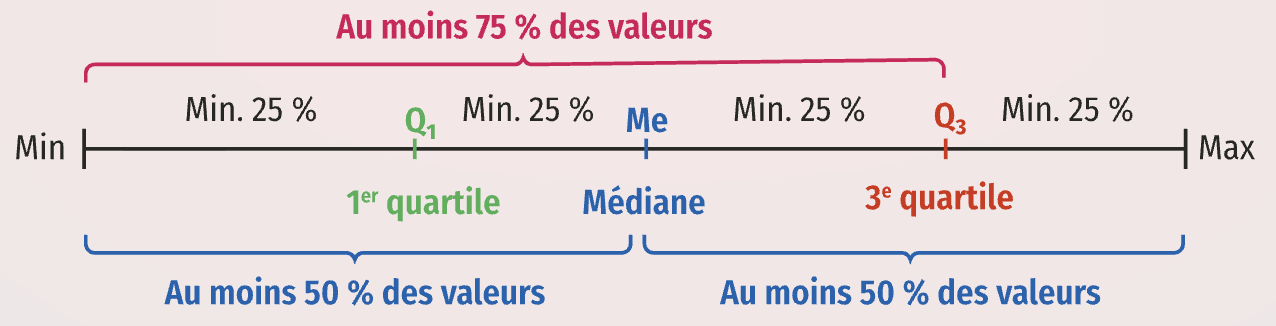
\includegraphics[width=0.8\textwidth]{fig1.png}    
\end{center}

\end{mdframed}

\vspace{10pt}
\underline{Exemple :}

\vspace{5pt}
On reprend la série précédente : -2 ; -1 ; 0 ; 0 ; 3 ; 4 ; 4 ; 5 ; 15 ; 25.

\vspace{20pt}
On calcule d'abord le \textbf{rang} de $Q_1$ : {\color{black!45}\dotfill}

\vspace{20pt}
Ce qui correspond à la \_\_\_\_\_\_\_ valeur : $Q_1 = $

\subsection*{\hspace{1cm} 3) L'écart interquartile : un indicateur de dispersion }
\vspace{5pt}

\begin{mdframed}[
    linewidth=1pt,
    roundcorner=5pt,
    linecolor=ForestGreen,
    innertopmargin=10pt,
    innerbottommargin=10pt
]
{\color{ForestGreen}
\textbf{\underline{Définition :}}}

\vspace{5pt}
\begin{itemize}
    \item L'\textbf{écart interquartile} est la différence $Q_3 - Q_1$
    \item L'\textbf{intervalle interquartile} est l'intervalle $\left[Q_1;Q_3\right]$
\end{itemize}

\end{mdframed}

\begin{mdframed}[
    linewidth=1pt,
    roundcorner=5pt,
    linecolor=Red,
    innertopmargin=10pt,
    innerbottommargin=10pt
]
{\color{red}
\textbf{\underline{Propriété :}}

\vspace{5pt}
Au moins \textbf{50\% des valeurs} de la série sont comprises dans l'\textbf{intervalle interquartile}.
}
\end{mdframed}

\begin{mdframed}[
    linewidth=1pt,
    roundcorner=5pt,
    linecolor=RoyalBlue,
    innertopmargin=10pt,
    innerbottommargin=10pt
]
{\color{RoyalBlue}
\textbf{\underline{Exercice d'application n°2:} Calculer les indicateurs d'une série.}}

\vspace{5pt}
On rappelle les notes obtenues par Nadir et Julie : 

\vspace{5pt}
Nadir : 4, 6, 18, 8, 17, 11, 12, 10

\vspace{5pt}
Julie : 15, 9, 14, 13, 10, 12, 12, 11, 10

\vspace{5pt}
\hspace{1cm}1) Calculer la moyenne puis la médiane de chacun.e 

\hspace{1cm}2) Calculer les quartiles puis l'écart interquartile.

\vspace{0.5cm}
{\color{black!45}\dotfill}

\vspace{0.5cm}
{\color{black!45}\dotfill}

\vspace{0.5cm}
{\color{black!45}\dotfill}

\vspace{0.5cm}
{\color{black!45}\dotfill}

\vspace{0.5cm}
{\color{black!45}\dotfill}

\vspace{20pt}

\end{mdframed}

\vspace{10pt}
\section*{\textcolor{red}{II/ Moyenne pondérée et écart-type}}

\vspace{5pt}
\subsection*{\hspace{1cm} 1) Moyenne pondérée}
\vspace{5pt}

\begin{mdframed}[
    linewidth=1pt,
    roundcorner=5pt,
    linecolor=ForestGreen,
    innertopmargin=10pt,
    innerbottommargin=10pt
]
{\color{ForestGreen}
\textbf{\underline{Définition :}}}

\vspace{5pt}
La \textbf{moyenne pondérée} $\bm{\overline{x}}$ d'une série dont les valeurs sont $x_1$, $x_2$, ..., $x_p$ et 
les effectifs correspondants $n_1$, $n_2$, ..., $n_p$ est égale à : 
\[
\overline{x} = \dfrac{n_1x_1 + n_2x_2 + ... + x_p}{n_1 + n_2 + ... + n_p}
\]

\end{mdframed}

\begin{mdframed}[
    linewidth=1pt,
    roundcorner=5pt,
    linecolor=RoyalBlue,
    innertopmargin=10pt,
    innerbottommargin=10pt
]
{\color{RoyalBlue}
\textbf{\underline{Exercice d'application n°3:} Calculer une moyenne pondérée.}}

\vspace{5pt}
Un super professeur de mathématiques (moi par exemple) a recensé les notes sur 5 de ses élèves de seconde obtenues 
lors de la première interrogation de l'année.

\vspace{-5pt}
\begin{center}
    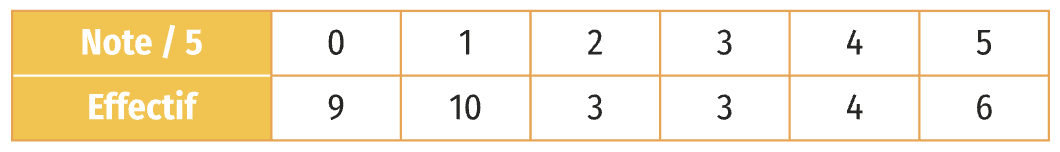
\includegraphics[width=0.65\textwidth]{fig2.png}
\end{center}

\vspace{-10pt}
\hspace{1cm}Calculer la moyenne pondérée de la classe.

\vspace{0.5cm}
{\color{black!45}\dotfill}

\vspace{0.5cm}
{\color{black!45}\dotfill}

\vspace{0.5cm}
{\color{black!45}\dotfill}

\vspace{0.5cm}
{\color{black!45}\dotfill}

\vspace{0.5cm}
{\color{black!45}\dotfill}

\vspace{0.5cm}
{\color{black!45}\dotfill}

\vspace{0.5cm}
{\color{black!45}\dotfill}


\vspace{20pt}


\end{mdframed}

\vspace{5pt}
\subsection*{\hspace{1cm} 2) Variance et écart-type : un indicateur de dispersion}
\vspace{5pt}

\begin{mdframed}[
    linewidth=1pt,
    roundcorner=5pt,
    linecolor=ForestGreen,
    innertopmargin=10pt,
    innerbottommargin=10pt
]
{\color{ForestGreen}
\textbf{\underline{Définition :}}}

\vspace{5pt}
\textbullet \hspace{0.1cm}La \textbf{variance} $\bm{V}$ d'une série de valeurs $x_1$, $x_2$, ..., $x_p$, de moyenne $\overline{x}$ et 
d'effectifs $n_1$, $n_2$, ..., $n_p$ est définie par :

\[
V = \dfrac{n_1(x_1 - \overline{x})^2 + n_2(x_2 - \overline{x})^2
+ ... + n_p(x_p - \overline{x})^2}{n_1 + n_2 + ... + n_p}
\]

\vspace{10pt}
\textbullet \hspace{0.1cm}L'\textbf{écart-type} d'une série de valeurs, noté $\bm{\sigma}$ est égale à :

\vspace{-5pt}
\[
\sigma = \sqrt{V}
\]

\end{mdframed}

{\color{red}\textbf{\underline{À RETENIR :}}} l'\textbf{écart-type} représente la dispersion 
des valeurs de la série autour de sa moyenne.

\vspace{15pt}
Plus l'écart-type est \_\_\_\_\_\_\_\_\_\_\_\_, plus les valeurs sont \_\_\_\_\_\_\_\_\_\_\_\_
\_\_\_\_\_\_\_\_

\vspace{15pt}
\_\_\_\_\_\_\_\_\_\_\_\_\_\_\_\_\_\_\_\_\_\_\_\_

\vspace{20pt}
\begin{mdframed}[
    linewidth=1pt,
    roundcorner=5pt,
    linecolor=RoyalBlue,
    innertopmargin=10pt,
    innerbottommargin=10pt
]
{\color{RoyalBlue}
\textbf{\underline{Exercice d'application n°4:} Calculer l'écart-type d'une série.}}

\vspace{5pt}
En reprenant les résultat de la classe du super professeur sympa, calculer l'écart-type des notes de la 
classe.

\vspace{0.5cm}
{\color{black!45}\dotfill}

\vspace{0.5cm}
{\color{black!45}\dotfill}

\vspace{0.5cm}
{\color{black!45}\dotfill}

\vspace{0.5cm}
{\color{black!45}\dotfill}

\vspace{0.5cm}
{\color{black!45}\dotfill}

\vspace{0.5cm}
{\color{black!45}\dotfill}

\vspace{0.5cm}
{\color{black!45}\dotfill}

\vspace{0.5cm}
{\color{black!45}\dotfill}

\vspace{20pt}

\end{mdframed}




\end{document}
